%% analyse.tex
%% $Id: analyse.tex 61 2012-05-03 13:58:03Z bless $
% !TEX root = thesis.tex

\chapter{Analyse und Evaluierung}
\label{ch:AnalyseUndEvaluierung}
%% ==============================

Die Beantwortung der Leitfrage des Projekts, ob durch Quantified Self das Wohlbefinden verbessert werden kann, hängt maßgeblich von einer genauen Analyse der Daten ab. 
Die zuvor in der Datengenerierungsphase erhobenen Daten müssen unter Berücksichtigung etwaiger Fremdeinflüsse bzw. Verfälschungen analysiert und ausgewertet werden.
Um dies zu gewährleisten sind wichtige Anforderungen an die Analyse gestellt, auf die im Folgenden näher eingegangen wird.

Exemplarische wurden nun nachdem alle Daten analysiert und ausgewertet wurden eine Testperson ausgewählt, anhand der die Leitfrage „Lässt sich das Wohlbefinden durch Quantified Self verbessern?“ beantwortet werden soll.

Aufgrund einer in der Gesamtheit Neuerhebung von Daten, liegt bei deren Auswertung der Fokus auf der deskriptive Datenanalyse.

\begin{quote}
\textit{„Deskriptive Datenanalyse: Liegt eine Totalerhebung oder generell ein Datensatz vor, so ist es die Aufgabe der Datenanalyse, die in den Einzeldaten enthaltene Information zu verdichten und diese so darzustellen, dass Wesentliches deutlich wird. Dazu werden Tabellen, graphische Darstellungen und charakteristische Maßzahlen verwendet.  Die Datenanalyse hat ausschließlich beschreibenden Charakter (deskriptive Statistik).“} 
\end{quote}
\cite[Springer Gabler Wirtschaftslexikon]{web:SpringerDatenanalyse}


Laut Schäfer\cite{Schafer2010} ist im Anschluss der deskriptiven Datenanalye mit der explorativen Statistik fortzufahren.
Dabei wird versucht Muster zu erkennen, welche mit Hilfe von Grafiken und Daten beschrieben werden.
Abschließend wird mit der Inferenzstatistik die Auswertung vollendet.
In diesem letzten Schritt wird versucht mit Hilfe von Stichprobendaten auf die allgemeine These zu schließen.

Dazu wurden verschiedene Korrelationskoeffizienten berechnet und Graphen erstellt.


%% ==============================
\section{Zusammenhang Schlafqualität und Schritte pro Tag}
%% ==============================
\label{ch:AnalyseUndEvaluierung:sec:ZusammenhangSchlafqualitätProSchrittenAmTag}


Das Diagramm \ref{fig:ZusammenhangSchlafqualitätProSchrittenAmTag} zeigt die Anzahl der aufgenommen Schritte pro Tag und zusätzlich die Schlafqualität in Prozent des jeweiligen Tages.
Die Werte der Grafik beziehen sich auf den kompletten Aufzeichnugszeitraums. 
Dabei handelt es sich bei den grünen Punkten um die einzelnen Datenpunkte der Schlafqualität, welche in Prozent auf der rechten Abzissenachse angegeben ist.
Auf der linken Abzissenachse wiederum wird die gesamte Anzahl der Schritte gezeigt, wie es auch der Legende zu entnehmen ist.
Zur besser Trend Ersichtlichkeit sind beide Datenreihen zusätzlich in einem Polynom sechsten Grades angenähert.
Diese Werte sind über den Erhebungszeitraum dargestellt.

Die Daten stammen aus dem Monat Mai des Jahres 2014.
In der Abbildung stamme die Werte Schritte pro Tag aus der im Projekt verwendeten Applikation Moves[\ref{ch:Apps:sec:Moves}]. 
Sleep Cycle[\ref{ch:Apps:sec:SleepCycle}] liefert dabei die Daten zur Schlafqualität.
Die Werte wurden im Zuge des Projektes von den Autoren erhoben.

\begin{figure}[H]
\centering
        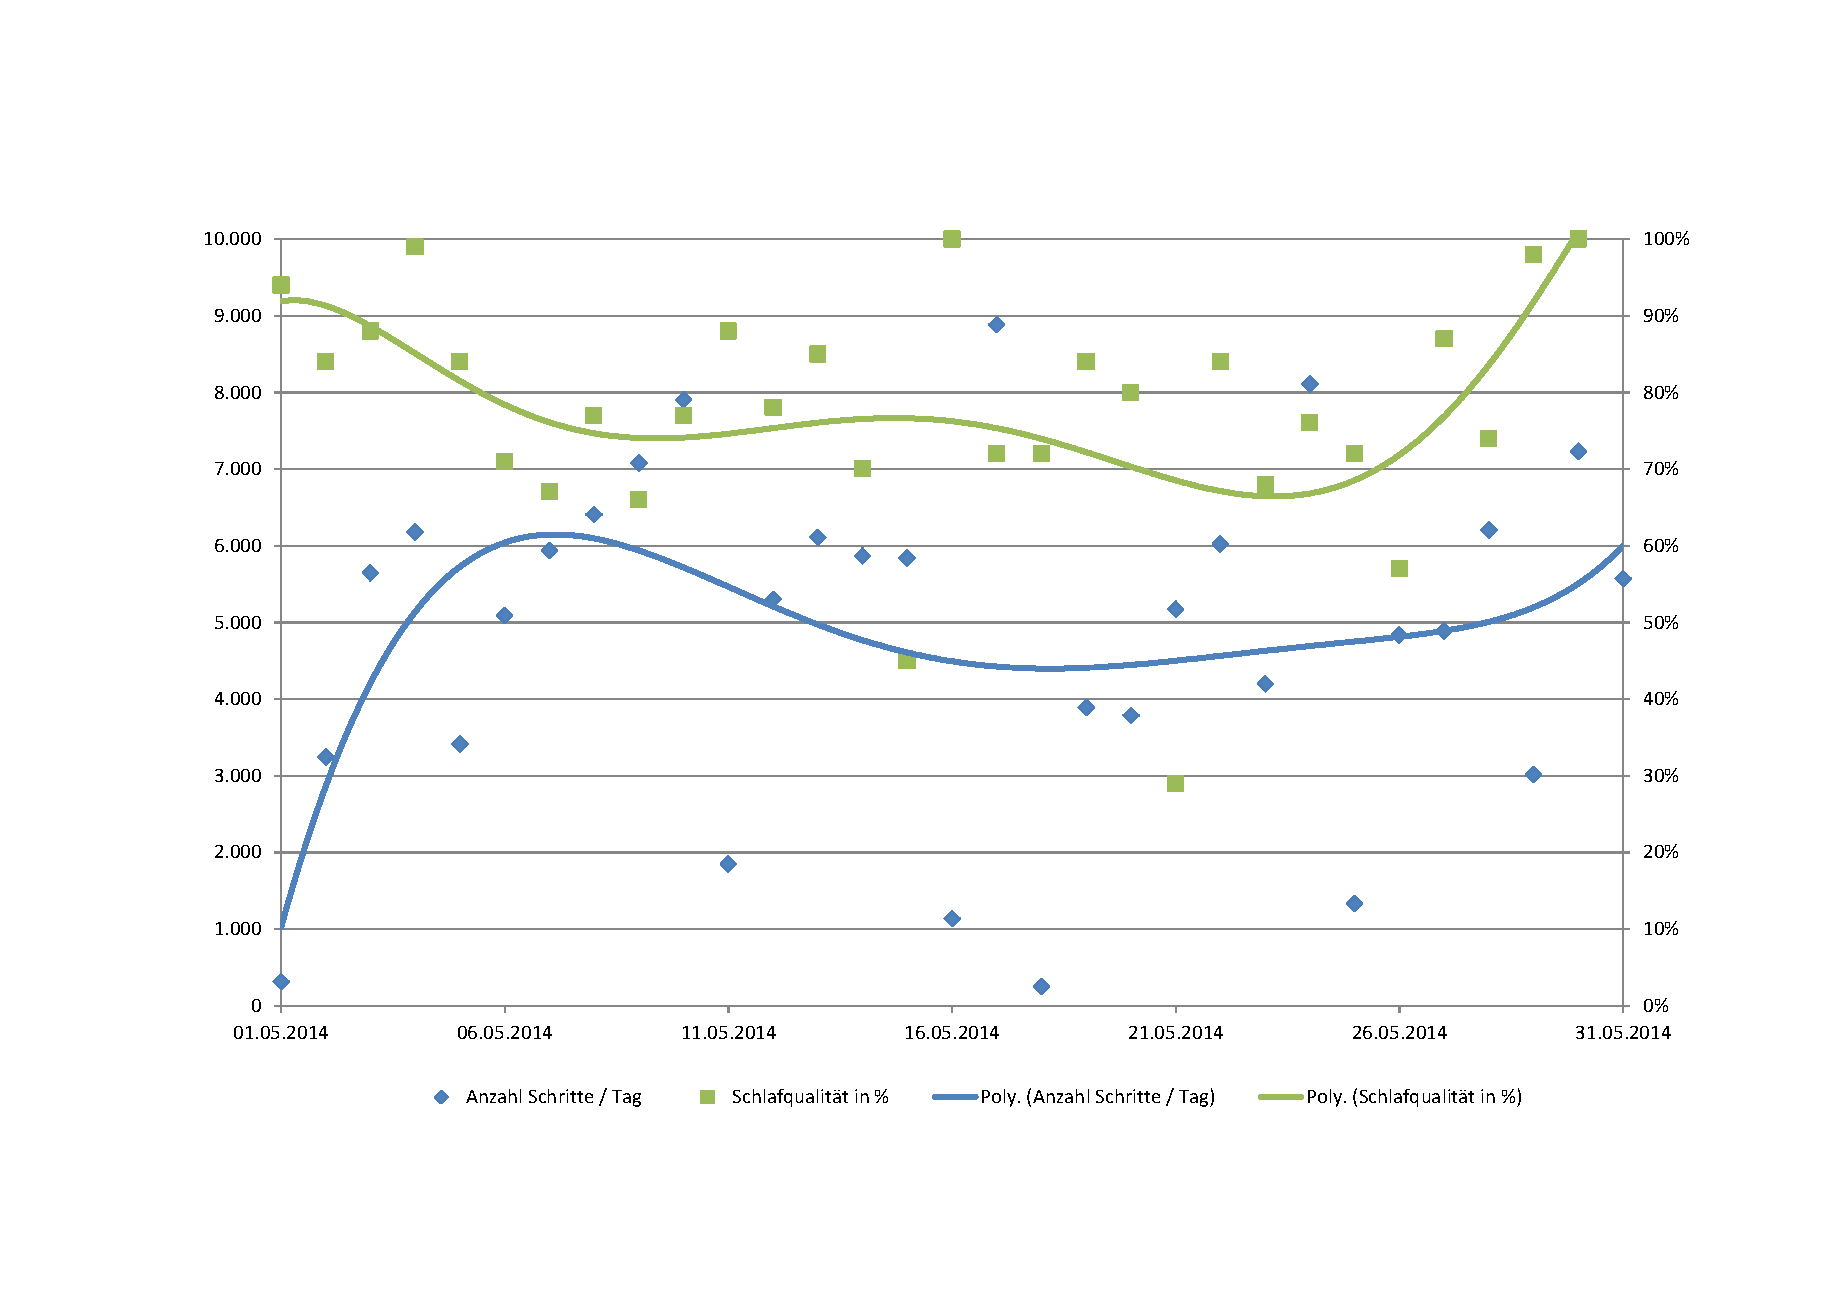
\includegraphics[angle=270,width=0.8\textwidth]{images/Analyse/Sleep-Steps} 
        \caption[Daten der Schritte pro Tag und der Schlafqualität]{Daten der Schritte pro Tag und der Schlafqualität}
        \label{fig:ZusammenhangSchlafqualitätProSchrittenAmTag}
\end{figure}




%% ==============================
\section{Zusammenhang von Stimmung, Schlafqualität und Energieverbrauch}
%% ==============================
\label{ch:AnalyseUndEvaluierung:sec:KorrelationVonSchlafqualitätUndSchrittenAmTag}

\begin{figure}[H]
\centering
        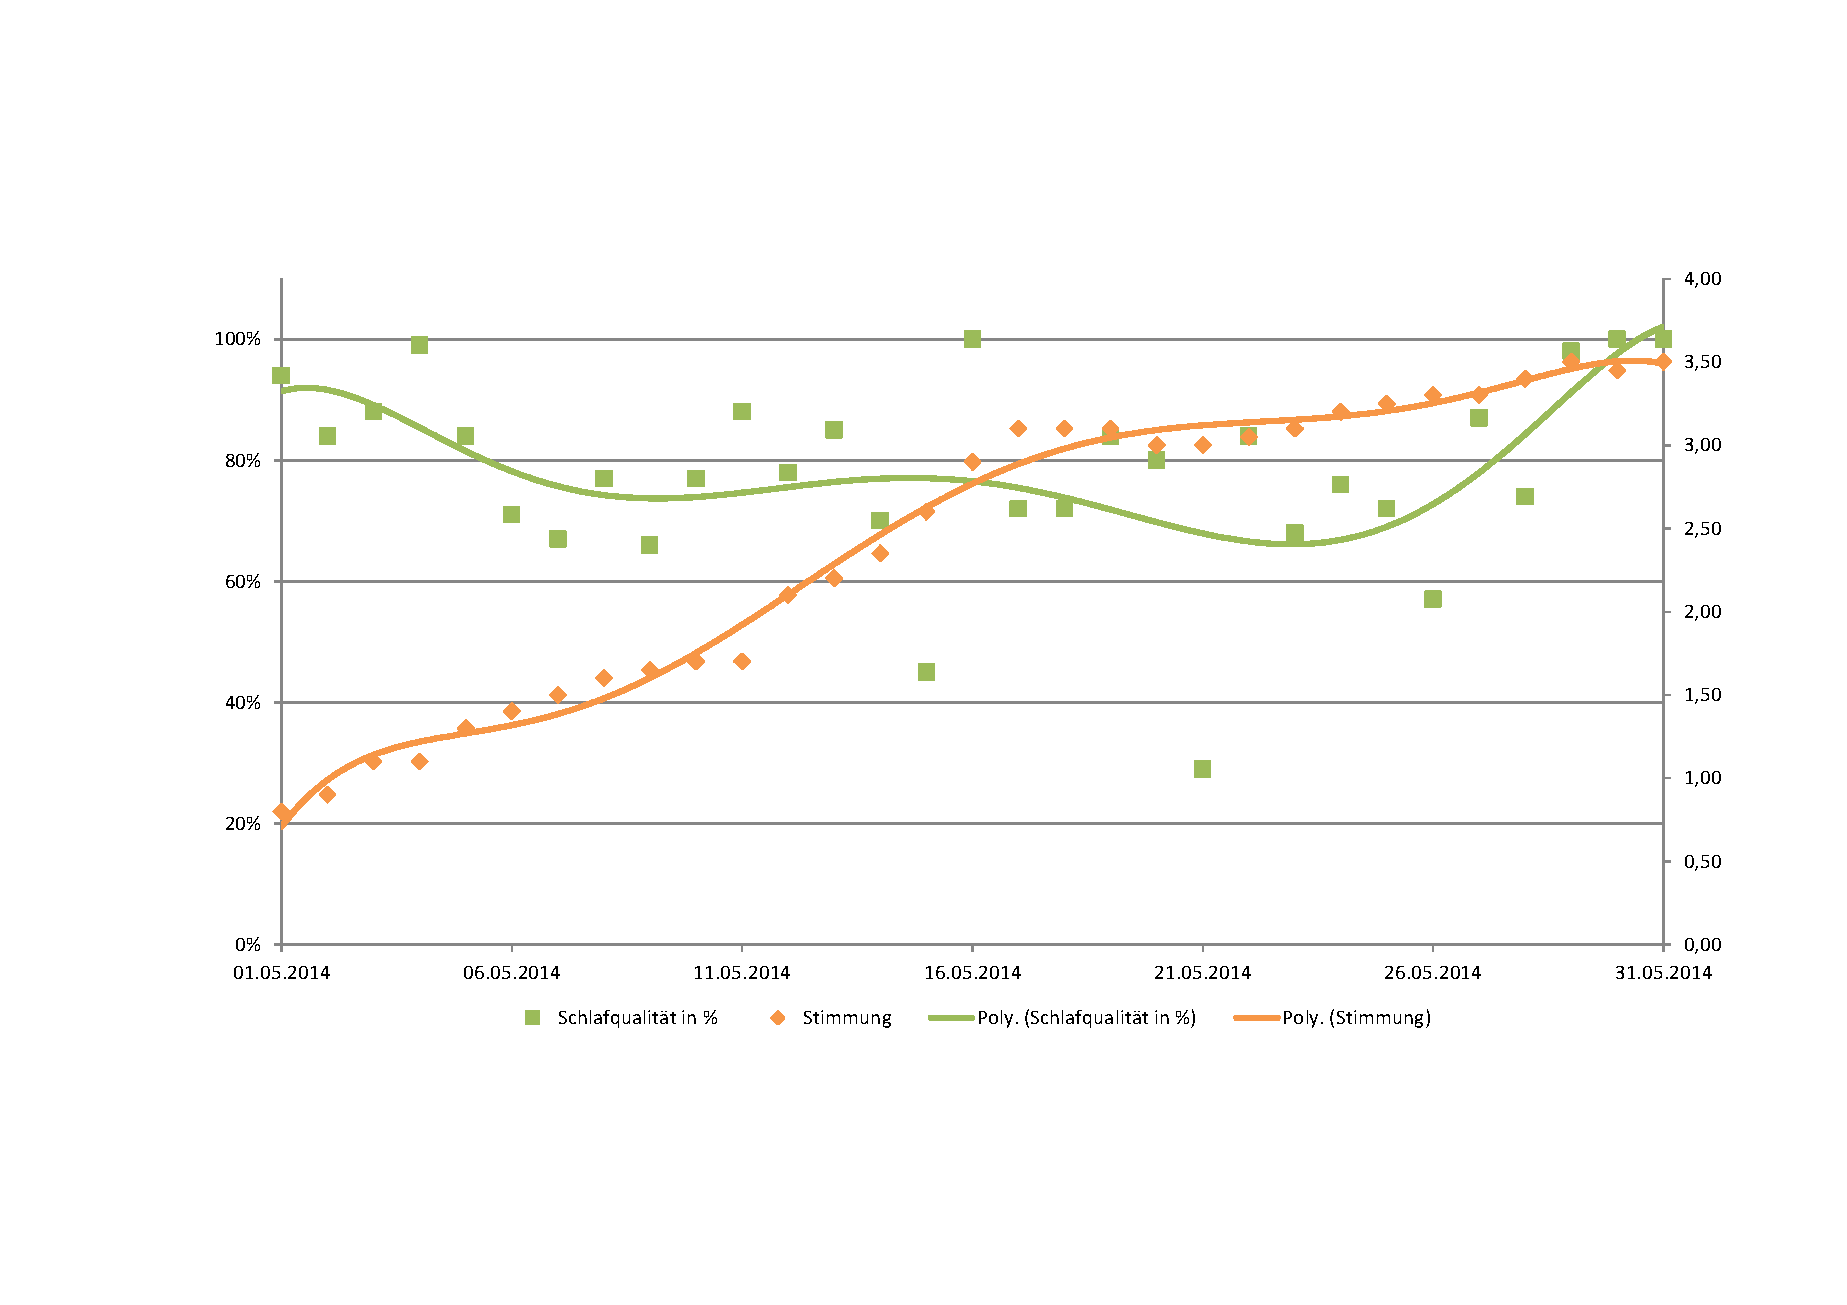
\includegraphics[angle=270,width=0.8\textwidth]{images/Analyse/Sleep-Mood} 
        \caption[Daten der Stimmung und der Schlafqualität]{Daten der Stimmung und der Schlafqualität}
        \label{fig:ZusammenhangVonStimmungUndSchlafqualität}
\end{figure}

%% ==============================
\section{Zusammenhang von Schlafqualität und Schritten am Tag}
%% ==============================
\label{ch:AnalyseUndEvaluierung:sec:KorrelationVonSchlafqualitätUndSchrittenAmTag}

\begin{figure}[H]
\centering
        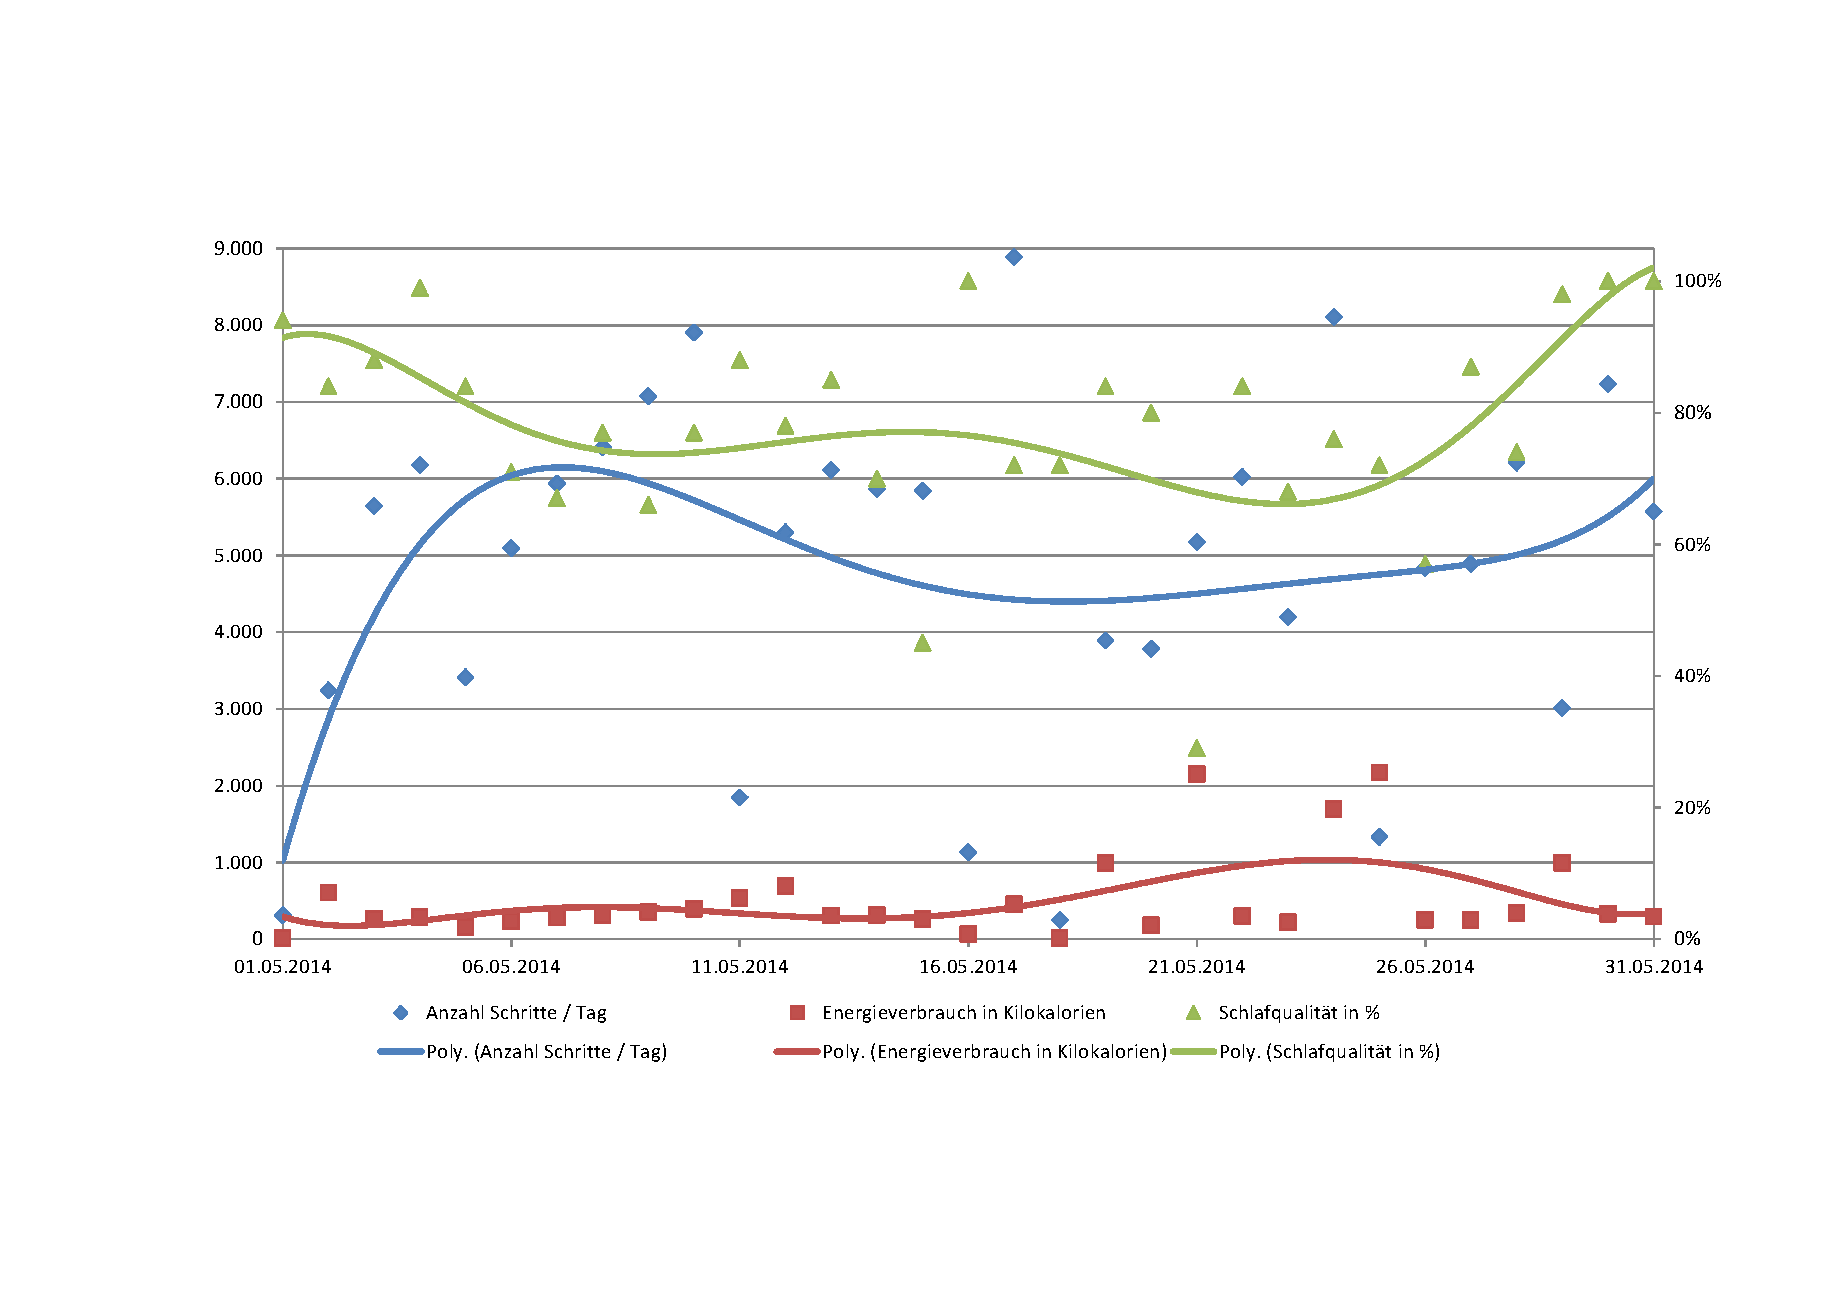
\includegraphics[angle=270,width=0.8\textwidth]{images/Analyse/Sleep-Steps-kcal} 
        \caption[Daten der Stimmung, der Schlafqualität und des Energieverbrauchs]{Daten der Stimmung, der Schlafqualität und des Energieverbrauchs}
        \label{fig:ZusammenhangVonSchlafqualitätSchrittenUndEnergieverbrauchAmTag}
\end{figure}

%% ==============================
\section{Zusammenfassung}
%% ==============================
\label{ch:Analyse:sec:zusammenfassung}


Diese Analyse liefert auf Basis einer ausführlichen Datenanalyse mit den gängigen Verfahren der Datenanalyse und -auswertung, der zuvor gewonnenen Daten, ein sehr exaktes Bild über die Zusammenhänge der jeweiligen Aktivitäten.
Die graphische Darstellung orientiert sich strikt an der Leitfrage des Projekts. 
Dadurch erhält der Leser eine erste Orientierung in welche Richtung die Beantwortung der Leitfrage ziehlen wird.

%% inferenzstatistik kann => nicht applyable weil nicht repräsentativ, referenzieren auf relativierung

%%% Local Variables: 
%%% mode: latex
%%% TeX-master: "thesis"
%%% End: 
